% RoGS-SLAM — MMM 2027 submission (Springer LNCS).
%
% Build: ./build.sh  ->  build/main.pdf, 14 pages (12 body + 2 references).
%
% Files: main.tex (this file) + body.tex + references.bib (29 entries) +
%        llncs.cls + splncs04.bst. Figures in ../figures/.
% This package is self-contained: nothing outside this directory is needed.
%
% Note: MMM 2027 has no supplementary-material channel; the SI is kept
% separately in ../supplementary/ for internal use only.
\documentclass[a4paper]{llncs}

\usepackage[T1]{fontenc}
\usepackage{graphicx}
% figures live one level up; keep the generated body free of paths
\graphicspath{{figures/}}
\usepackage{amsmath}
\usepackage{booktabs}
\usepackage{array}
\usepackage{url}
\usepackage{cite}
\usepackage{needspace}

% Float placement: the body's [t] figures are page-scale; with LaTeX's default
% \topfraction=0.7 a figure plus its long caption exceeds the top-area budget
% and every following float defers to the end of the document. Relax the caps
% so figures place at (or near) their source page.
\renewcommand{\topfraction}{0.95}
\renewcommand{\bottomfraction}{0.95}
\renewcommand{\textfraction}{0.05}
\renewcommand{\floatpagefraction}{0.85}
\setcounter{topnumber}{3}
\setlength{\emergencystretch}{1.5em}
\setcounter{totalnumber}{5}

% Tighter float separation: keeps Sec. 7 Conclusion on page 12 so that the
% reference-only allowance (max 2 pages) starts cleanly on page 13.
\setlength{\textfloatsep}{4pt plus 1pt minus 1pt}
\setlength{\abovecaptionskip}{2pt}
\setlength{\floatsep}{6pt plus 2pt minus 2pt}
\abovedisplayskip=5pt plus 1pt minus 1pt
\belowdisplayskip=5pt plus 1pt minus 1pt
\abovedisplayshortskip=3pt plus 1pt minus 1pt
\belowdisplayshortskip=3pt plus 1pt minus 1pt

\begin{document}

\title{RoGS-SLAM: Robust Gaussian Splatting SLAM in Dynamic
Environments via Reliability-Guided Weighting}
\titlerunning{RoGS-SLAM: Robust Gaussian Splatting SLAM in Dynamic Environments}
\author{Bin Chen\inst{1}
\and
Jie Su\inst{1}\thanks{Corresponding author}
\and
Jing Zhang\inst{2}\thanks{Corresponding author}}
\authorrunning{Bin Chen et al.}
\institute{School of Information Science and Engineering, University of Jinan, Jinan 250022, China\\
\email{chenb5@stu.ujn.edu.cn}, \email{ise\_suj@ujn.edu.cn}
\and
Yantai Institute of Science and Technology, Yantai 265600, China\\
\email{ise\_zhangjing@ujn.edu.cn}}

\maketitle

\begin{abstract}
A moving object supplies residuals that a rigid-world estimator resolves by moving the
camera. Run unmodified, our 3D-Gaussian-splatting (3DGS) SLAM backbone drifts to 39--147 cm,
against roughly 1.5 cm on static scenes. The dominant response detects movers with an
external, class-conditioned network and discards them. We instead decide which pixels to
trust from the disagreement between observed optical flow and the flow a rigid scene
would produce, down-weighting rather than removing, and report the measurements that
bound the result. A pre-registered 120-run factorial over three of its four components
finds component necessity \emph{regime-dependent}; no sequence demonstrably rewards all
three, so the full bundle is nowhere strictly necessary. A controlled counterpart given
the same frozen flow improves on the baseline on only 2 of its 4 held-out sequences and
is worse on one; our weighting improves on all four. Three pose-side endpoints expose a
variance--bias trade that forces pose claims to name their endpoint. On the crowd scenes
our combined (masked) configuration leads the RGB-D 3DGS class we reproduce under one
protocol (2.2--2.3 cm ATE) at 4.0 GB, against 7.4 for RGD-SLAM. We give the per-frame
observable marking where the mask-free configuration stops being sufficient.

\keywords{Dynamic SLAM \and 3D Gaussian splatting \and Scene reconstruction \and Robust estimation.}
\end{abstract}

% Body of the MMM 2027 submission. Edit this file directly.

\section{Introduction}


A moving object supplies photometric and geometric residuals that a rigid-world estimator resolves by moving the camera. Run unmodified, our 3DGS-SLAM backbone drifts to 39.3 cm on the mixed-mover sequence \texttt{balloon} and 147.5 cm on a crowded one, against roughly 1.5 cm on static scenes. The dominant response detects the movers and removes them. An external, class-conditioned network labels which pixels could move, and the estimator discards them (Sec. 2.1). It works, but it makes the dynamic decision a per-frame classification by a second model, with its cost and failure modes; and it is closed-set, which bites hardest on user-generated content, where the label set is open. Recent lines replace the \emph{class} prior with a learned uncertainty (Sec. 2.2) or move the decision out of the segmentation network (Sec. 2.3).


Our configuration sits in that third line. It decides which pixels to trust from \emph{consistency}, the disagreement between observed optical flow and the flow a rigid scene would produce, and it down-weights rather than removes. Operating without semantic segmentation is not itself a contribution we claim, since prior work has done that. Two kinds of evidence are missing. One shows which of its parts are necessary, and on which sequences. The other separates the mechanism's own effect from the extra information a method was handed.


We present RoGS-SLAM, a mask-free core for dynamic 3DGS-SLAM. On the crowd scenes it tracks at 2.2--2.3 cm where the backbone drifts to 86--147 cm, at 4.0 GB of GPU memory, without any category label. Its contributions are the measurements that bound this result:


\begin{enumerate}\setlength{\itemsep}{0pt}
\item \textbf{Component necessity is regime-dependent, and we measured it rather than asserting it.} A pre-registered three-factor factorial (8 cells $\times$ 5 sequences $\times$ 3 seeds = 120 runs) leaves no sequence on which all three components are supported (0 of 5), so the full bundle is nowhere strictly necessary, and the useful subset is a function of the regime (Sec.~5.2).

\item \textbf{The gain is not attributable to the information alone.} Under an equal, strictly causal budget on the byte-identical frozen flow, a naive per-pixel threshold stably improves on the baseline on only 2 of 4 held-out sequences and is worse on \texttt{pt2} (51.07 vs 45.37 cm). Our mechanism improves on 4 of 4 (1.63--4.99$\times$) and beats the naive counterpart on all four (Sec. 5.4), closing the ``it just had more information'' reading.

\item \textbf{The pose-side mechanism is a variance--bias trade, measured on the intermediate quantity.} One single-variable intervention, extending the semantic hard tracking mask of the \emph{combined} configuration from 10 to all 100 tracking iterations, moves the per-frame dynamic penalty worse (+0.0806 cm, 1.22$\times$ its noise floor) yet full-trajectory error better ($-$1.42 cm, 4.0$\times$). This rests on one sequence with two legs near their floors (Sec. 5.6). The consequence generalises beyond this system. A pose-side claim must name its endpoint.
\end{enumerate}


The same evidence delimits where the mask-free configuration is not sufficient (Sec. 5.5).




\section{Related Work}


\subsection{Dynamic SLAM built on explicit dynamic priors}


Dynamic SLAM has long followed \emph{detect-then-exclude}. DynaSLAM~\cite{dynaslam}, NGD-SLAM~\cite{ngdslam} and RoDyn-SLAM~\cite{rodynslam} segment or detect movers with Mask R-CNN~\cite{maskrcnn}, YOLO, and fused flow and segmentation masks. The pattern is widespread in 3DGS dynamic SLAM: RGD-SLAM~\cite{rgdslam} uses a pre-trained OneFormer, DG-SLAM~\cite{dgslam} initialises poses from DROID-VO~\cite{droidslam}, and BDGS-SLAM~\cite{bdgsslam}, DAGS-SLAM~\cite{dagsslam} and DynaGSLAM~\cite{dynagslam} build per-Gaussian priors from YOLO or SAM2~\cite{sam2} detections. In every case the dynamic decision is delegated to an external, class-conditioned model, with the costs named in Sec.~1.


\subsection{Replacing the class prior with a learned uncertainty}


WildGS-SLAM~\cite{wildgsslam} drops the category prior while keeping a learned one: per-pixel uncertainty from ``a pre-trained DINOv2 feature extractor'' and metric depth ``as estimated by Metric3D v2''. Its own overview defines \emph{Prior Free} as ``not using class priors''; we apply the same standard to ourselves. Our label is \emph{mask-free}, never \emph{prior-free}, and it, too, keeps a pretrained network (the frozen RAFT flow of Sec. 3.4).


\subsection{Dynamic decisions from consistency rather than from categories}


A third line keeps a segmentation or depth network but moves the dynamic decision out of it, with pre-3DGS roots. ReFusion~\cite{bonn} rejects dynamic residual pixels in a purely geometric RGB-D pipeline with no learned prior at all. Recent 3DGS systems refine the move with learned front ends: Gassidy~\cite{gassidy} decides which YOLO instances move by analysing rendering-loss flows, DGS-SLAM~\cite{dgsslamkong} pairs an online Track-Anything segmentation with a photometric-consistency mask, Dy3DGS-SLAM~\cite{dy3dgsslam} fuses an optical-flow mask with a DepthanythingV2 depth mask, and GARAD-SLAM~\cite{garadslam} states that ``we do not perform semantic segmentation on the feature points in the tracking phase''. Our configuration belongs to this line (Sec.~1). What it does that these do not is keep the decision continuous: the disagreement between observed and rigid flow becomes a bounded per-pixel weight that never removes a pixel, and the same signal also weights the density lifecycle. The line shows that ``mask-free'' must be checked per system: of these four, two still consume a segmentation network and a third a monocular depth network.


The ingredients we combine are each individually classical. Robust M-estimation~\cite{huber}, residual reweighting, and keyframe management all have ample precedent. Our backbone, MonoGS~\cite{monogs}, ``maintain[s] a small window W\_k'' of keyframes and performs no loop closure, and the systems of Secs.~2.1--2.3 are its SLAM-side descendants, down to SplaTAM~\cite{splatam} and Co-SLAM~\cite{coslam} in Table~1. What is missing is not another robust kernel but the measurements Sec.~1 named.




\section{Method}


RoGS-SLAM adds four components to a 3DGS-SLAM backbone, none of them a new primitive. This section states what each one changes in the estimator, so the ablations of Sec. 5 read as interventions on named quantities. Constants are resolved from the run configuration.


\subsection{Backbone and attachment points}


The backbone is MonoGS~\cite{monogs} in its RGB-D configuration: the frontend estimates each frame's pose against a fixed 3D Gaussian splatting scene~\cite{3dgs}, and the backend re-optimises Gaussian parameters and the poses of a bounded keyframe window. We change neither the representation nor the rasteriser, but we do change the density lifecycle. Four components attach at four distinct places and a fifth is optional (Fig.~1): \textbf{uniform keyframe coverage (K)} decides which frames become keyframes, \textbf{robust reweighting (R)} how much each pixel's residual counts in the pose solve, the \textbf{reliability signal (L)} which pixels are trusted as static, and the \textbf{lineage lifecycle (D)} which newly created Gaussians survive; the optional semantic person mask of Sec.~3.6 supplies a fifth. The \emph{mask-free} configuration disables it, the \emph{combined} one enables it; no number obtained with the mask supports a statement about the mask-free system.


\begin{figure}[t]\centering
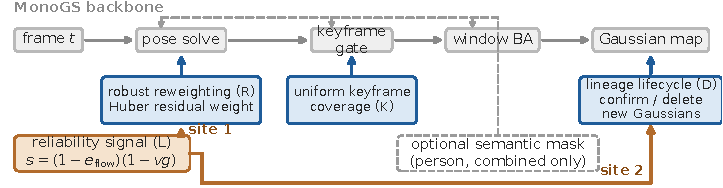
\includegraphics[width=\textwidth]{fig1_pipeline.pdf}
\caption{\emph{Where the components attach.} Grey boxes are the backbone. Blue and orange boxes modify the stage their arrow points into. Dashed grey is the optional semantic mask with its three consumers: the mapping loss, the keyframe-insertion gate, and the warm-up-only hard tracking mask (Sec. 5.6). }\end{figure}


\subsection{Coverage: uniform temporal keyframe sampling}


MonoGS selects keyframes adaptively by co-visibility, so density is a property of the scene; across our five ablation sequences it spans 0.045 to 0.075 keyframes per frame. Coverage adds one rule. More than \texttt{gap\_cap = 5} frames since the last keyframe force an insert, and the native criterion is floored rather than replaced. Density becomes near-constant at 0.198 to 0.204 keyframes per frame, at a cost of 2.7--4.5$\times$ more keyframes and roughly double the map size.


\subsection{Robust reweighting: Huber IRLS inside the pose solve}


R leaves the L1 tracking objective of the backbone in place and adds an iteratively-reweighted least-squares step~\cite{zhang} on top of it. For residual $r$ the weight is the standard Huber~\cite{huber} IRLS weight $w_{\text{rob}}(r) = \min(\delta/|r|, 1)$ with $\delta = 0.1$ per channel. It is computed from a detached residual and recomputed at every tracking iteration, so the weights co-adapt with the pose, unlike the fixed per-frame map of Sec. 3.4. The weight multiplies the per-pixel residual, and the residual is then averaged over the summed weight rather than over the pixel count, $L = \alpha\,\frac{\sum w_{rgb}\,v\,|I-\hat I|}{\sum w_{rgb}} + (1-\alpha)\,\frac{\sum w_{d}\,|D-\hat D|}{\sum w_{d}}$ with $\alpha = 0.9$, $v$ the rendered opacity, and both sums over pixels valid in that channel. Weights therefore renormalise which pixels contribute; they do not rescale the objective, and an all-equal weighting reproduces the unmodified loss. A pre-registered ablation (6 sequences $\times$ 2 alternative kernels $\times$ 3 seeds = 36 runs) supports Huber over the two other kernels the codebase implements; neither is better outside the pre-registered floor, and both degrade on \texttt{pt2} by 1.8 and 2.5 cm.


\subsection{Reliability: a per-frame, per-pixel static-confidence map}


This component consumes optical flow and decides, without any category label, which pixels count as evidence about camera motion (Fig.~2); Fig.~3 shows what this leaves in the final map. Each frame needs the frozen backward flow, the rendered depth and opacity at the warmed-up pose, and the observed depth. The pose used to predict rigid flow is the tracker's own current estimate after \texttt{warmup\_iters} iterations, not a reference or ground-truth pose.


\begin{figure}[t]\centering
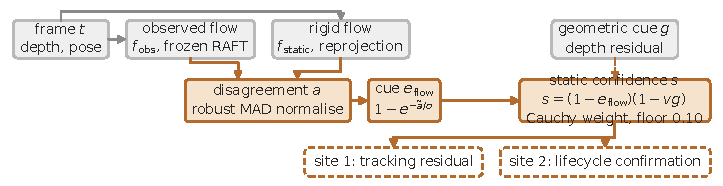
\includegraphics[width=\textwidth]{fig2_reliability.pdf}
\caption{\emph{The reliability signal, from flows to weights (Sec.~3.4).} Observed flow and rigid reprojection flow disagree on movers; a per-frame robust MAD normaliser turns that disagreement into $e_{\text{flow}}$, which fuses with the depth-residual cue $g$ into the static confidence $s$ and the floored Cauchy tracking weight. Equations in Sec.~3.4.}\end{figure}


\textbf{Observed and rigid flow.} For frame $t$ we take a precomputed backward flow $f_{\text{obs}} = f_{t \to t-1}$ from a frozen RAFT~\cite{raft} and the rigid-flow prediction $f_{\text{static}}$ from reprojection through the current depth and ego-motion. The mover shows up in that disagreement, though so can occlusion boundaries and flow error, which the robust normaliser of the next step absorbs.


\textbf{Threshold-free normalisation.} Let $a = \|f_{\text{obs}} - f_{\text{static}}\|_2$ over valid pixels and write $\tilde a = [a - \operatorname{median}(a)]_+$. The cue is $e_{\text{flow}} = 1 - \exp\!\big(-\tilde a / (\sigma + \varepsilon)\big)$ with $\sigma = \max(1.4826\,\operatorname{MAD}(a),\, \texttt{floor})$ and $\texttt{floor} = 2.0$ px. The floor matters because $\operatorname{MAD}$ collapses to zero on a near-static frame, where the score would otherwise saturate on flow noise; 2.0 px was calibrated on a static sequence as the robust noise floor of $a$. Pixels with non-finite or out-of-bounds flow are excluded rather than scored zero.


\textbf{Combining the cues.} The geometric cue is the same normaliser applied to the axial depth residual, $g = 1 - \exp\!\big(-[r_d - \operatorname{median}(r_d)]_+ / (1.4826\,\operatorname{MAD}(r_d) + \varepsilon)\big)$ with $r_d = |D - \hat D|$ over pixels where both depths are finite and positive. It is gated by the rendered opacity $v$ so unmapped regions cannot vote, and the two cues fuse into the static confidence $s = (1 - e_{\text{flow}})(1 - vg)$. A pixel is trusted only if both cues find it unremarkable, and $s \to 1$ recovers the unmodified estimator. With $d = 1 - s$ the tracking weight is a frame-adaptive Cauchy down-weight


\begin{equation}
w_{\text{rel}} = \frac{1}{1 + (d/\tau)^2}, \qquad
\tau = \operatorname{median}(d) + 1.4826\,\operatorname{MAD}(d) + \varepsilon
\end{equation}


where the knee $\tau$ is a Hampel-type robust z-score; the same normaliser that defines $e_{\text{flow}}$ prices deviation from the frame's own $d$ distribution.


\begin{figure}[t]\centering
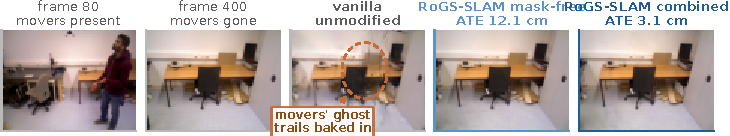
\includegraphics[width=\textwidth]{fig3_map_comparison.pdf}
\caption{\emph{What each configuration bakes into the final map.} The first two panels are the observed scene at frame 80, person mid-sequence, and at frame 400 after both movers left. The last three are each arm's final map rendered at frame 400 from its own pose. The backbone's map is shredded by ghost trails (circled); both RoGS-SLAM arms reconstruct the static office, the mask-free one without any class label. The two arms look alike here because they differ in tracking stability, not map appearance. Post-hoc offline renders, for illustration, not a benchmark metric.}\end{figure}


\textbf{The weight is bounded away from zero.} What multiplies the residual is $\max(w_{\text{rel}}, 0.10)$, so a pixel is attenuated by at most 10$\times$ and never removed. This is the sharpest difference from a mask and the comparison Sec. 5.4 leans on.


\textbf{When it is computed, and where it is consumed.} The map is computed once per frame after \texttt{warmup\_iters = 10} tracking iterations and then frozen; without frozen flow, $w_{\text{rel}} \equiv 1$ and the estimator is unchanged. It is consumed at two sites: at the \textbf{tracking residual}, $\max(w_{\text{rel}}, 0.10)$ multiplies the Huber weight of Sec. 3.3 in both channels, and at \textbf{candidate confirmation} in the lifecycle of Sec. 3.5, $s$ weights the evidence. The ablation removes this pair of interventions sharing one signal.


\textbf{Where the robust knee breaks.} $\tau$ is a \emph{majority} statistic. A mover occupying a large share of the frame joins the population that sets its own knee, which is one reason the mask stays dominant on mixed-mover sequences (Sec. 5.1).


\subsection{The density lifecycle}


The backbone commits every new Gaussian immediately; we replace that rule with an evidence test. Each Gaussian created at a keyframe carries a \textbf{lineage} identifier, and every later keyframe that sees it re-projects it. With $\tau_d = \max(0.03\,\text{m}, 0.02\hat z)$ and $\delta = z - \hat z$ between observed and projected depth, a view \emph{supports} the lineage if $|\delta| \le \tau_d$ and the mean absolute colour difference is at most 0.15, \emph{contradicts} it if $\delta > \tau_d$, and is \emph{occluded} if $\delta < -\tau_d$ (neither). Observations need finite positive $z$ outside any semantic-mask pixel, and views with no valid flow are gated out when reliability is enabled, so a missing cue is never read as static. Evidence accumulates as $C^{+}{=}\sum s\,h$ over supporting and $C^{-}{=}\sum s$ over contradicting views, with $h = \mathrm{clip}(1-|\delta|/\tau_d,0,1)$. A lineage is promoted at $C^{+} \ge 2 \wedge C^{+} > C^{-}$, rejected in full at $C^{-} \ge 2 \wedge C^{-} > C^{+}$, and expired after 5 unconfirmed keyframes; without reliability the same test uses integer counts. The replacement is materially active (median 0.55 of created lineages are deleted), so a comparison against stock MonoGS compares a different density rule.


\subsection{The optional semantic mask, and the simpler configuration}


In the \emph{combined} configuration a Mask R-CNN~\cite{maskrcnn} person mask (dilated by 7 px) reaches three consumers: the \textbf{mapping loss}, the \textbf{keyframe-insertion gate}, and the \textbf{tracking residual}. The last is a hard mask only for the first \texttt{warmup\_iters} tracking iterations, after which the soft weight of Sec.~3.4 takes over the person region. Switching between \emph{mask-free} and \emph{combined} opens these paths inside \emph{this} component only, never the reliability signal, and holding the hard mask on for all tracking iterations (the intervention of Sec.~5.6) shows the two cues compose rather than replace each other. The attribution campaign uses a third, \emph{simpler} configuration (native sparse keyframes, robust reweighting, the lifecycle, and the mask applied only at the mapping loss) relative to which \emph{combined} flips four switches, not three: uniform coverage, reliability, insertion-gate masking, and the warm-up hard tracking mask. Sec.~5.3 measures the first two in isolation and Sec.~5.6 varies the fourth. All sixteen constants, one of them a disclosed-inert threshold, are resolved from the run configuration.




\section{Experimental Protocol}


Decisions below were frozen before the campaigns of Sec. 5 ran.


\textbf{Sequences.} 18 RGB-D sequences (8 BONN~\cite{bonn}, 10 TUM RGB-D~\cite{tumrgbd}), spanning static, low-motion, high-motion and \emph{object-only} scenes. The denominator is fixed, no campaign may select a subset after seeing results, and the object-only movers carry no person label.


\textbf{Trajectory accuracy.} Full-trajectory absolute-trajectory error (ATE) RMSE (cm) via \texttt{evo}~\cite{evo} after SE(3) Umeyama alignment~\cite{umeyama} without scale correction. ATE covers all frames, and we also report the relative pose error (RPE, translation, per frame).


\textbf{Seeds and completion.} Every configuration runs with 3 seeds (mean $\pm$ sd, spreads reaching 2$\times$ flagged). A run counts as completed only at $\ge$ 95\% of frames, and a pair with fewer than two co-completed seeds is \emph{unresolved}, not dropped.


\textbf{Rendering, efficiency, hardware.} Rendering metrics are computed offline from the final map, and refinement does not touch the reported trajectory. Efficiency is reported from the online phase and compared only on identical hardware. Flow is precomputed by a frozen RAFT~\cite{raft} network, so RAFT inference is not in the online rate (Sec. 5.7). All campaigns ran on an RTX 3090, and each reported cell maps to exactly one run directory. The pre-registration record, the resolved configuration of every arm, the eight factorial cells with their per-seed ATE and completion status, the cue-split factorial, the RPE held-out runs and the complete 18-sequence table ship with the source archive under \texttt{evidence/}, so each number in Secs.~4--5 can be traced to a run.




\section{Results}


\subsection{Trajectory accuracy under one protocol (Table 1)}


\textbf{On the crowd scenes, combined tracks at 2.3/2.2 cm where the unmodified backbone drifts to 86.5/147.5 cm.} Table~1 compares all reproduced methods on four BONN dynamic scenes under one protocol. Crowd is the mask-dominant regime; combined is the best RGB-D 3DGS configuration there, yet two CPU-side systems with no dense map average lower, and the mask-free arm stays 34.9/45.9. On the object-only scene the segmentation-free arms are unaffected while DynaGSLAM pays for its person-only detector; on \texttt{pt2} combined trails both WildGS-SLAM and DG-SLAM, and mask-free is the better of our own two arms.


\begin{table}[t]\centering\scriptsize\setlength{\tabcolsep}{2pt}
\begin{tabular}{>{\raggedright\arraybackslash}p{3.3cm}rrrrrr}\toprule
Method & crowd & crowd2 & mv\_no\_box & pt2 & Avg. & GPU (GB) \\ \midrule
\multicolumn{7}{l}{\emph{Ours, dynamic 3DGS}} \\
RoGS-SLAM combined (ours) & 2.3$\pm$0.0 & 2.2$\pm$0.1 & 2.7$\pm$0.1 & 10.4$\pm$0.8 & 4.4 & 4.0$\pm$1.0 \\
RoGS-SLAM mask-free (ours) & 34.9$\pm$28.3 & 45.9$\pm$17.4 & 3.1$\pm$0.5 & 9.3$\pm$0.6 & 23.3 & 3.4$\pm$1.0 \\
\midrule
\multicolumn{7}{l}{\emph{Dynamic 3DGS}} \\
RGD-SLAM & 2.6$\pm$0.3 & 2.4$\pm$0.1 & 2.3$\pm$0.3 & 23.0$\pm$3.7 & 7.6 & 7.4$\pm$1.1 \\
DG-SLAM & 5.8$\pm$0.1 & 6.4$\pm$0.5 & 3.0$\pm$0.1 & 6.1$\pm$0.1 & 5.3 & 7.3$\pm$0.4 \\
DynaGSLAM & 23.8$\pm$0.0 & 13.7$\pm$0.0 & 12.1$\pm$0.0 & 13.7$\pm$0.0 & 15.8 & 2.2$\pm$0.7 \\
WildGS-SLAM (mono) & {\boldmath$1.55\pm0.06$} & {\boldmath$2.17\pm0.05$} & {\boldmath$1.6\pm0.0$} & {\boldmath$3.1\pm0.0$} & 2.1 & 12.1$\pm$1.9 \\
\midrule
\multicolumn{7}{l}{\emph{Dynamic, non-3DGS}} \\
RoDyn-SLAM (NeRF) & 5.6$\pm$0.2 & 4.6$\pm$0.1 & 16.5$\pm$7.1 & 14.4$\pm$0.1 & 10.3 & 1.0$\pm$0.1 \\
DynaSLAM (CPU) & 2.1$\pm$0.2 & 2.8$\pm$0.3 & 2.3$\pm$0.1 & 8.8$\pm$1.2 & 4.0 & --- \\
NGD-SLAM (CPU) & 1.8$\pm$0.2 & 2.2$\pm$0.1 & 2.0$\pm$0.1 & 6.6$\pm$0.4 & 3.2 & --- \\
\midrule
\multicolumn{7}{l}{\emph{Static}} \\
SplaTAM & 135.4$\pm$36.1 & 493.2$\pm$470.7 & 37.4$\pm$0.4 & 132.7$\pm$9.4 & 199.7 & 6.9$\pm$7.4 \\
MonoGS (unmodified) & 86.5$\pm$18.3 & 147.5$\pm$39.0 & 15.3$\pm$9.5 & 43.8$\pm$8.6 & 73.3 & 0.5$\pm$0.2 \\
Co-SLAM (implicit) & div. & div. & 10.1$\pm$0.3 & 71.3$\pm$2.9 & 40.7 & 1.1$\pm$0.0 \\
ORB-SLAM3 (sparse) & 76.6$\pm$27.9 & 111.4$\pm$14.8 & 24.9$\pm$5.9 & 76.8$\pm$2.1 & 72.4 & --- \\
\bottomrule\end{tabular}
\caption{ATE RMSE (cm, mean $\pm$ sd, 3 seeds) on four BONN dynamic scenes, grouped by representation and dynamic handling. Every row, competitors included, is our own reproduction under one protocol. \emph{combined} is the full system and \emph{mask-free} its core without the semantic mask. \textbf{Bold} marks the lowest ATE per column; Avg and GPU are unranked since they mix modalities and hardware; div.\ = diverged. Only ours and RGD-SLAM share one RTX 3090, so the GPU column is comparable within that pair alone.}\end{table}


\textbf{Where the mask matters, measured between our own two arms.} The ratio $N = \text{ATE}_{\text{mask-free}} / \text{ATE}_{\text{combined}}$ never passes through the vanilla denominator, so it is quotable wherever both arms ran. On the six BONN sequences beyond the crowd pair, the mask is redundant on \texttt{mv\_no\_box2}, \texttt{mv\_no\_box} and \texttt{pt2} (0.89--1.17$\times$) and dominant on \texttt{balloon2}, \texttt{pt1} and \texttt{balloon} (1.92--3.96$\times$). Sec. 5.5 tracks this split with a per-frame observable across all 18 sequences.


\subsection{Component necessity is regime-dependent (Fig. 4)}


The pre-registered factorial varies K, R, and L (8 cells $\times$ 5 sequences $\times$ 3 seeds = 120 runs). It runs mask-free, with D pinned identically in all cells. Writing the removal effect of component $f$ on sequence $s$ as


\begin{equation}
\Delta_f(s) = E[\log \text{ATE} \mid f \text{ removed}, s] - E[\log \text{ATE} \mid \text{full}, s]
\end{equation}


positive $\Delta_f$ means removing $f$ hurts, so the two questions are global necessity ($\Delta_f(s) \ge 0\ \forall s$) and full-bundle reward ($\Delta_f(s) \ge 0\ \forall f$). With 3 seeds per cell neither receives an inferential answer, so we apply a descriptive support rule. A cell supports a component only where $|\text{mean}| \ge 1$ sd; cells failing it (marked $\circ$ in Fig.~4) are directional, not negative. Under this rule neither necessity reading is established. $\Delta_L$ is positive on 5 of 5 sequences (the only component with that property, though 3 of the 5 cells are directional), and no sequence has all three components supported (0 of 5), so the full bundle is nowhere strictly necessary across the five measured sequences. Crowd is absent from this factorial; its evidence is the crowd2 ladder of Sec. 5.3.


\begin{figure}[t]\centering
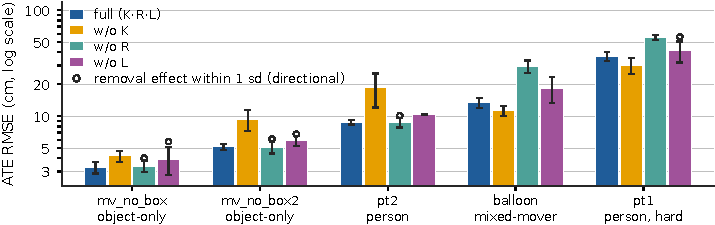
\includegraphics[width=\textwidth]{fig4_component_necessity.pdf}
\caption{\emph{Component necessity is regime-dependent.} ATE RMSE (cm, log scale) of the full mask-free configuration and of the three single-component removals, per sequence, from the pre-registered factorial (8 cells $\times$ 5 sequences $\times$ 3 seeds). Bars are 3-seed means with $\pm$1 sd. $\circ$ marks a removal whose mean log-shift is within 1 sd of its own seed spread, i.e.\ directional only.}\end{figure}


$\Delta_K > 0$ strongly on the object-only sequences and \texttt{pt2} yet $\Delta_K < 0$ on \texttt{balloon} and \texttt{pt1}. $\Delta_R$ is not distinguishable from zero at three seeds on the three easier sequences yet is the largest effect in the matrix on \texttt{balloon} (+0.780$\pm$0.037). $\Delta_L$ is the only one never negative (5/5), costing 1.19--1.34$\times$ on \texttt{pt2} and \texttt{balloon}. When L is off, both of its consumption sites go off with it (site 2 reverts to integer counts), so $\Delta_L$ is the joint effect of L's two sites (Sec. 3.4). A two-by-two ablation over mask and coverage on \texttt{balloon} moves ATE fourfold along the mask axis and not at all along the coverage axis (3.06 vs 3.03 cm), so coverage is not the kernel. And a cue-split factorial finds geometry-only lower than the shipped fusion on 3 of 4 sequences, so fixed cue fusion is not universal.


\subsection{Single-variable attribution}


The full ladder is descriptive and covers two sequences (24 runs). On \texttt{mv\_no\_box}, coverage alone recovers the full arm's advantage (2.71$\pm$0.04 vs 2.63$\pm$0.09 cm, within the pre-registered floor). On \texttt{crowd2}, no tested subset comes close (coverage 5.16, reliability 6.00, pair 4.55, insertion gating 5.66, full 2.11 cm), so the crowd gain is attributed to the bundle. The 18-sequence denominator reads 2.19$\pm$0.09 (crowd2) and 2.65$\pm$0.12 (mv\_no\_box), inside the drift discipline (we budget $\sim$30\%), and the 18-sequence campaign is canonical.


\subsection{The gain is not the flow information alone (Fig. 5a)}


To isolate the gain from the information, the counterpart consumes the same frozen backward flow, byte for byte, through a naive p90 threshold (frozen on pilot sequences) as a hard mask in place of our weighting. The control comprises 3 arms $\times$ 4 sequences $\times$ 3 seeds = 36 runs, rule fixed before the first.


The naive counterpart stably beats vanilla on only 2 of 4 under the all-seeds-same-sign rule and is worse on \texttt{pt2} (51.07 vs 45.37 cm); ours improves on all four (1.63--4.99$\times$) and beats the counterpart on all four. Every cell comes from the control's own campaign; the 18-sequence vanilla reading on \texttt{pt2} (43.85$\pm$8.55) differs inside the drift discipline of Sec.~5.3, so ratios divide same-campaign cells only. Across the three arms the keyframe rule, the robust kernel and its $\delta$, the density lifecycle and the optimisation budget are held identical; what differs is how the flow reaches the residual. The counterpart also lacks the MAD normaliser and geometric cue and removes rather than down-weights, so this control rules out the information alone and not every flow-consuming treatment.


\subsection{Where mask-free stops being sufficient (Fig. 5b)}


We test whether the mask-free arm's own per-frame RPE tracks that split. Across all 18 sequences, necessity is read as $N$ ($N \ge 1.5$ necessary, $N \le 1.2$ redundant).


The groups do not overlap, spanning 0.222--1.572 against 1.717--2.980 cm/frame. Every threshold in between separates all 17 decided sequences. \texttt{f3\_st\_hf} and \texttt{crowd} have nearly identical mask-free ATE yet $N$ values differing 12.6-fold. Per-frame drift tracks mask necessity, and accumulated error does not.


\begin{figure}[t]\centering
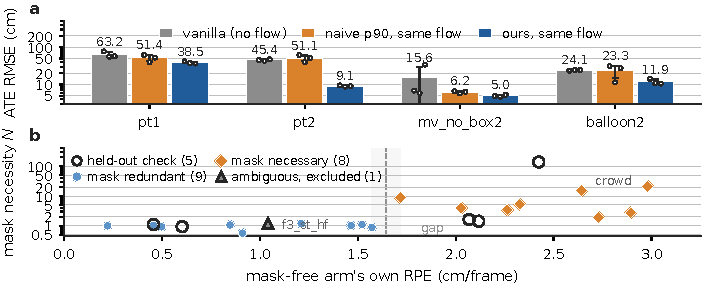
\includegraphics[width=0.72\textwidth]{fig5_controlled_comparison.pdf}
\caption{\emph{Two controlled comparisons.} (a) ATE RMSE (cm, log scale) when the same byte-identical frozen flow is consumed by nothing, by a naive p90 threshold, or by our weighting; dots are seeds, bars 3-seed means ($\pm$1 sd). (b) Mask necessity $N$ against the mask-free arm's own per-frame RPE. The grey band is the empirical gap, the dashed line the pre-registered midpoint $\tau$, and black-edged markers the first-round held-out checks.}\end{figure}


\textbf{Scope of the interval.} It requires running the mask-free arm, so it is a post-hoc diagnosis, not a selector. The pre-registered midpoint $\tau = 1.6445$ cm/frame was tested on two rounds of unseen sequences (5, then 6, all outside the denominator), with the ambiguity band the open interval $(1.2, 1.5)$ and $N \le 0.8$ the frozen-sense line. One first-round sequence lands in the band and is undecidable, leaving 10 decided, of which 8 agree in direction and both misses are conservative. No RPE fell inside the band, so its location is untested.


\subsection{The pose-side mechanism}


\begin{figure}[b]\centering
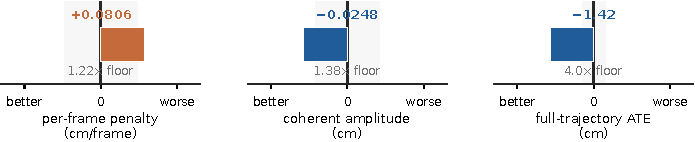
\includegraphics[width=0.95\textwidth]{fig6_pose_endpoints.pdf}
\caption{\emph{One intervention, three pose-side endpoints, opposite signs (Sec.~5.6).} Shift on \texttt{balloon} from holding the semantic hard tracking mask on for all 100 tracking iterations instead of 10, in intervention-minus-control raw units per endpoint, with the grey band the $\pm$1 re-run noise floor of that endpoint.}\end{figure}


One intervention holds the semantic hard tracking mask of combined on for 100 tracking iterations instead of 10, with soft reliability retained on surviving static pixels. Three pose-side endpoints move in opposite directions (Fig.~6). The \emph{per-frame dynamic penalty}, median RPE on high-dynamic frame pairs minus that on low-dynamic pairs, moves worse (+0.0806 cm/frame, 1.22$\times$ floor). The \emph{coherent amplitude}, mean cosine similarity between consecutive RPE vectors times median $|$RPE$|$ on the high-dynamic pairs, moves lower ($-$0.0248 cm, 1.38$\times$). Full-trajectory ATE moves better ($-$1.42 cm, 4.0$\times$). The measurement is consistent with a variance--bias trade but rests on \texttt{balloon} alone, two legs near their floors. Writing $e_t=b_t+\varepsilon_t$ with zero-mean $\varepsilon_t$, suppressing pixels can raise per-frame noise while lowering the systematic pull that accumulates into drift. A tracking claim must therefore name its endpoint.


\subsection{Rendering and cost}


Combined runs at 0.75$\pm$0.09 FPS and 4.02$\pm$1.01 GB on the same RTX 3090, within one sd of mask-free (0.77$\pm$0.21, 3.43$\pm$0.99). Mask R-CNN runs online, cached per keyframe; precomputed RAFT is excluded, and adding it back (54 ms/frame) puts end-to-end tracking near 0.6 FPS, so 0.75 FPS is an online-phase rate, not a deployment rate. Across 18 sequences, post-hoc renders show full-frame PSNR ranking the ghost-carrying backbone above both arms (19.1 vs 18.8/18.6 dB), so PSNR is read as map self-consistency, never trajectory evidence; Depth-L1, the one rendering metric co-ordered with ATE, improves from 46.9 to 31.4--32.3 cm.




\section{Limitations}


\textbf{1. Where our arms lose.} On \texttt{pt1}, mask-free reaches 32.41$\pm$8.52 cm against the mask's 11.89$\pm$2.36 (\texttt{pt2} needs no mask). On four of the 18 sequences both arms are worse than the backbone, with \texttt{f3\_st\_hf} by an order of magnitude (35.59/29.43 vs 2.80 cm) and the others 1.1--2.8$\times$. All four are \emph{sitting} or near-static captures with no sustained mover for the signal to key on, and \texttt{f3\_st\_hf} adds translation against a close surface, which magnifies the $1/z$ term of item~3.


\textbf{2. Accuracy scope.} Combined trails the best RGB-D comparator by 1.0--1.7$\times$ on the walking and person sequences (\texttt{f3\_wk\_hf} 3.29 vs 3.25 for RGD-SLAM and \texttt{pt2} 10.45 vs 6.1 for DG-SLAM), and monocular WildGS-SLAM by 3.4$\times$ on \texttt{pt2}.


\textbf{3. Static scenes, and the mechanism behind them.} On Replica~\cite{replica}, outside the denominator, combined is worse and less stable than the backbone (\texttt{office0} 3.82$\pm$4.58 vs 0.368$\pm$0.012 cm), so use it only when no dynamic content is present. The same mechanism explains the sitting sequences of item~1. Rigid flow is predicted from the pose the tracker is still optimising, so its own pose error \emph{is} a flow residual: a translation error $\delta t$ induces about $f_x\delta t/z$ pixels, which at 0.8 m is already 3.3 px at $\delta t = 5$ mm against a 2.0 px floor. Movers inflate $\operatorname{MAD}$ and absorb this term; on a near-static frame $\operatorname{MAD}$ collapses onto the floor and the tracker's own error becomes the anomaly. The induced error scales as $1/z$, so it lands on the near, parallax-rich pixels: the correlation between $e_{\text{flow}}$ and depth flips from $+0.11$ under a ground-truth pose to $-0.58$ under a perturbed one, and down-weighting that field raises the residual, which down-weights harder. Feeding ground-truth relative poses to the rigid-flow prediction alone, with tracking unchanged, recovers \texttt{f3\_st\_hf} from 35.3 to 2.85 cm, which bounds any correction of this loop and identifies the loop rather than the scene as the cause.


\textbf{4. Operating conditions.} On 8/18 sequences baseline CV exceeds 20\%, so ratios are basin-dependent.


\textbf{5. Crowd attribution and scope.} The crowd gain is attributable to the bundle (Sec.~5.3). All evidence comes from one MonoGS implementation; the mechanism needs only a rendered depth and opacity, an observed depth, a pose and a place to apply a per-pixel weight (any dense RGB-D Gaussian SLAM supplies those), but the calibration is tied to this backbone's residual statistics and needs re-measuring elsewhere.




\section{Conclusion}
% Final content page sits 3 lines past the 12-page boundary and the llncs
% widow/club penalties (10000) lock the Conclusion paragraph's break point.
% A one-page enlargement of 4 lines closes the gap; same technique the
% bibliography already uses (main_v3.tex uses 12\baselineskip there).
\enlargethispage{3\baselineskip}


We presented RoGS-SLAM, a mask-free core for dynamic 3DGS-SLAM, and the measurements that bound it. Component necessity is regime-dependent, the gain does not follow from the information alone, and pose-side claims must name their endpoint. A mask-free cue selector is future work.






\bibliographystyle{splncs04}
% The reference list overflows the 2-page allowance by ~half a page; LNCS accepts
% a compact reference list. Body font size stays uniform -- only the bibliography
% is set in \small.
% \clearpage keeps the two reference-only pages clean: content ends on page 12
% (the Fig. 5 bottom float closes the page) and references start at the top of
% page 13.
\clearpage
\section*{Acknowledgements}
We thank the members of our laboratory for their generous GPU support during the experiments. This work was supported by the National Natural Science Foundation of China (Grant No. 52171310, Research on Drift Trajectory Prediction Method for Deep Sea AUVs).

\small\setlength{\itemsep}{0pt}
\bibliography{references}

\enlargethispage{12\baselineskip}
\end{document}
